\chapter{Incorporación de Bases de Datos de Alta Resolución}
\newpage
\begin{figure}[H]
	\centering
	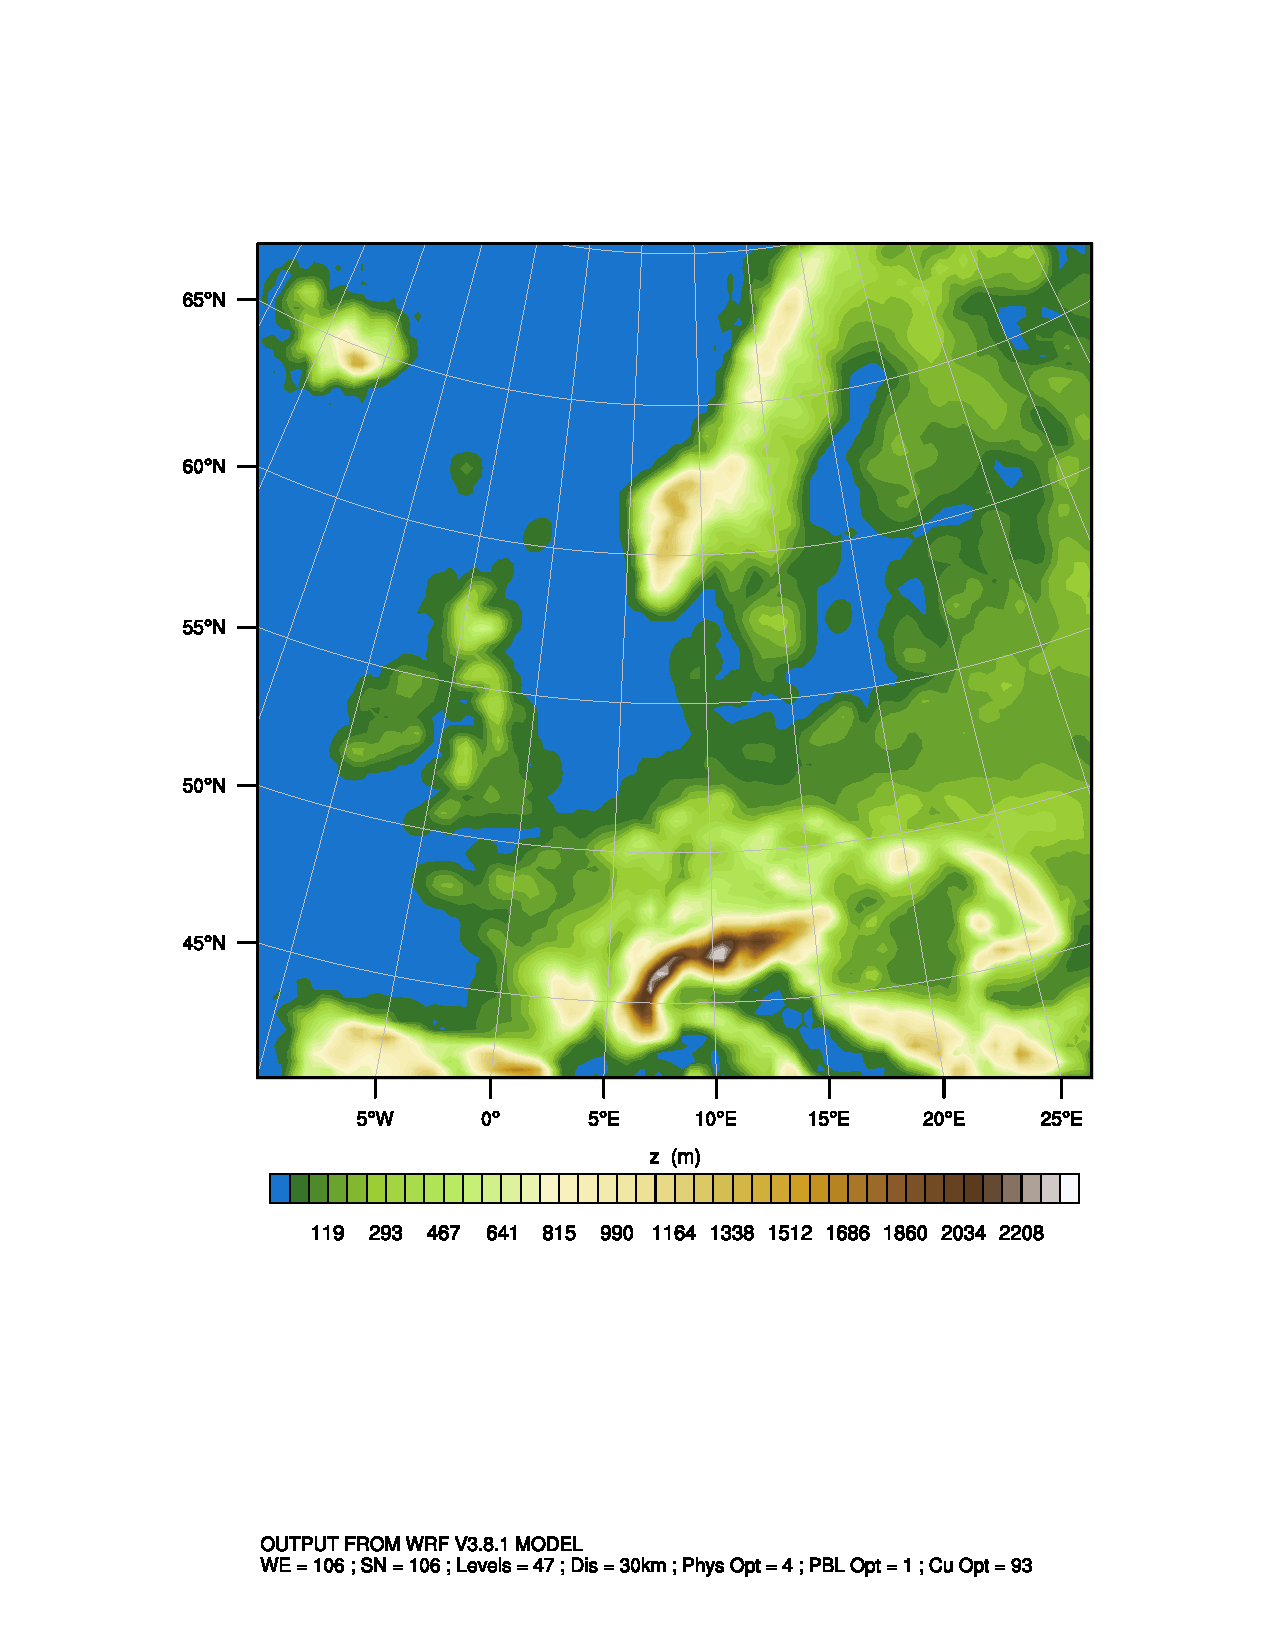
\includegraphics[width=0.25\linewidth,page=1,trim={2cm 6.5cm 1cm 3.5cm},clip]{Imagenes/05/hov_domain.pdf}%
	\includegraphics[width=0.25\linewidth,page=2,trim={2cm 6.5cm 1cm 3.5cm},clip]{Imagenes/05/hov_domain.pdf}%
	\includegraphics[width=0.25\linewidth,page=3,trim={2cm 6.5cm 1cm 3.5cm},clip]{Imagenes/05/hov_domain.pdf}%
	\includegraphics[width=0.25\linewidth,page=4,trim={2cm 6.5cm 1cm 3.5cm},clip]{Imagenes/05/hov_domain.pdf}%
	
	\bigskip
	\includegraphics[width=0.25\linewidth,page=5,trim={2cm 6.5cm 1cm 3.5cm},clip]{Imagenes/05/hov_domain.pdf}%
	\includegraphics[width=0.25\linewidth,page=6,trim={2cm 6.5cm 1cm 3.5cm},clip]{Imagenes/05/hov_domain.pdf}%
	\includegraphics[width=0.25\linewidth,page=7,trim={2cm 6.5cm 1cm 3.5cm},clip]{Imagenes/05/hov_domain.pdf}%
	\includegraphics[width=0.25\linewidth,page=8,trim={2cm 6.5cm 1cm 3.5cm},clip]{Imagenes/05/hov_domain.pdf}%
	
	\bigskip
	\includegraphics[width=0.25\linewidth,page=9,trim={2cm 6.5cm 1cm 3.5cm},clip]{Imagenes/05/hov_domain.pdf}%
	\includegraphics[width=0.25\linewidth,page=10,trim={2cm 6.5cm 1cm 3.5cm},clip]{Imagenes/05/hov_domain.pdf}%
	\includegraphics[width=0.25\linewidth,page=11,trim={2cm 6.5cm 1cm 3.5cm},clip]{Imagenes/05/hov_domain.pdf}%
	\includegraphics[width=0.25\linewidth,page=12,trim={2cm 6.5cm 1cm 3.5cm},clip]{Imagenes/05/hov_domain.pdf}%
	
	\bigskip
	\includegraphics[width=0.25\linewidth,page=13,trim={2cm 6.5cm 1cm 3.5cm},clip]{Imagenes/05/hov_domain.pdf}%
	\includegraphics[width=0.25\linewidth,page=14,trim={2cm 6.5cm 1cm 3.5cm},clip]{Imagenes/05/hov_domain.pdf}%
	
	\caption{Orografía (MSNM) y uso de suelo (categoría USGS24) de alta definición para cada uno de las mallas anidadas (d01-d07). Para el dominio d07 se presenta la ubicación del punto de control (rojo) y la distribución de turbinas eólicas en la zona (negro).}
	\label{fig:dominios}
\end{figure}

\begin{figure}[H]
	\centering
	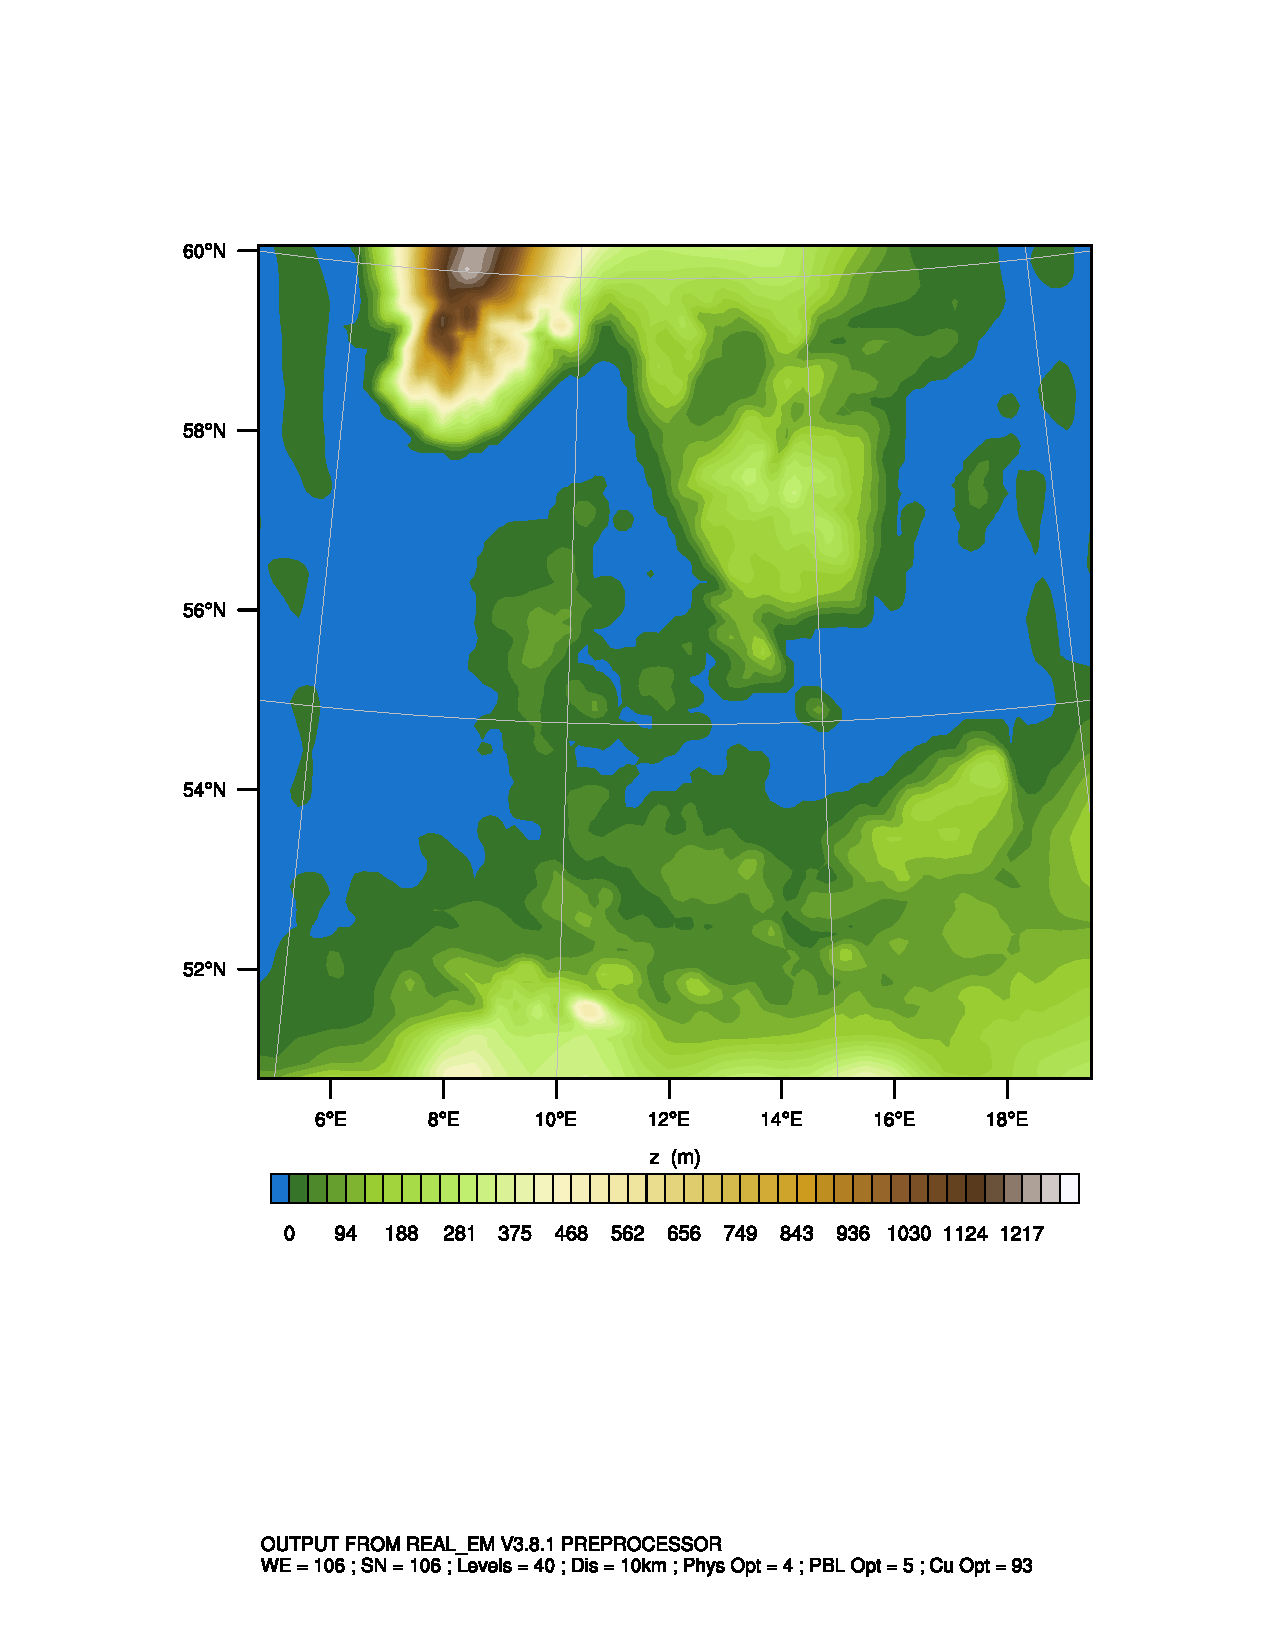
\includegraphics[width=0.25\linewidth,page=1,trim={2cm 6.5cm 1cm 3.5cm},clip]{Imagenes/05/bol_domain.pdf}%
	\includegraphics[width=0.25\linewidth,page=2,trim={2cm 6.5cm 1cm 3.5cm},clip]{Imagenes/05/bol_domain.pdf}%
	\includegraphics[width=0.25\linewidth,page=3,trim={2cm 6.5cm 1cm 3.5cm},clip]{Imagenes/05/bol_domain.pdf}%
	\includegraphics[width=0.25\linewidth,page=4,trim={2cm 6.5cm 1cm 3.5cm},clip]{Imagenes/05/bol_domain.pdf}%
	
	\bigskip
	\includegraphics[width=0.25\linewidth,page=5,trim={2cm 6.5cm 1cm 3.5cm},clip]{Imagenes/05/bol_domain.pdf}%
	\includegraphics[width=0.25\linewidth,page=6,trim={2cm 6.5cm 1cm 3.5cm},clip]{Imagenes/05/bol_domain.pdf}%
	\includegraphics[width=0.25\linewidth,page=7,trim={2cm 6.5cm 1cm 3.5cm},clip]{Imagenes/05/bol_domain.pdf}%
	\includegraphics[width=0.25\linewidth,page=8,trim={2cm 6.5cm 1cm 3.5cm},clip]{Imagenes/05/bol_domain.pdf}%
	
	\bigskip
	\includegraphics[width=0.25\linewidth,page=9,trim={2cm 6.5cm 1cm 3.5cm},clip]{Imagenes/05/bol_domain.pdf}%
	\includegraphics[width=0.25\linewidth,page=10,trim={2cm 6.5cm 1cm 3.5cm},clip]{Imagenes/05/bol_domain.pdf}%
	\includegraphics[width=0.25\linewidth,page=11,trim={2cm 6.5cm 1cm 3.5cm},clip]{Imagenes/05/bol_domain.pdf}%
	\includegraphics[width=0.25\linewidth,page=12,trim={2cm 6.5cm 1cm 3.5cm},clip]{Imagenes/05/bol_domain.pdf}%
	
	\bigskip
	\includegraphics[width=0.25\linewidth,page=13,trim={2cm 6.5cm 1cm 3.5cm},clip]{Imagenes/05/bol_domain.pdf}%
	\includegraphics[width=0.25\linewidth,page=14,trim={2cm 6.5cm 1cm 3.5cm},clip]{Imagenes/05/bol_domain.pdf}%
	
	\bigskip
	\includegraphics[width=0.25\linewidth,page=15,trim={0cm 6.5cm 1cm 3.5cm},clip]{Imagenes/05/bol_domain.pdf}%
	\includegraphics[width=0.25\linewidth,page=16,trim={0cm 6.5cm 1cm 3.5cm},clip]{Imagenes/05/bol_domain.pdf}%
	
	\caption{Orografía (MSNM) y uso de suelo (categoría USGS24) de alta definición para cada uno de las mallas anidadas (d01-d08).}
	\label{fig:c3dominios}
\end{figure}
